\section{Fixed Point}
Unsigned Interger Zahlen $z$ können mit $z=\sum_{k=0}^{n-1}a_k\cdot B^k$ berechnet werden. Signed Interger Zahlen mit $z=-(2^{n-1})\cdot a_{n-1}+\sum_{k=0}^{n-2}a_k\cdot B^k$, wobei $a_k$ die jeweilige Stelle der Bit Zahl entspricht. Um nun Fixed Points zu berechnen, wird das Q-Format verwendet. Dabei steht s/u für singed/unsigend und Qn.m für n=Integer bzw. m=fractional.

\textbf{Beispiel} $10110100$ entspricht im Format uQ2.6:
\[
1\cdot 2^1 + 0\cdot2^0 + 1\cdot2^{-1}+ 1\cdot2^{-2}+ 0\cdot2^{-3}+ 1\cdot2^{-4} = 2.8125
\]
und im Format sQ2.6:
\[
-1\cdot 2^1 + 0\cdot2^0 + 1\cdot2^{-1}+ 1\cdot2^{-2}+ 0\cdot2^{-3}+ 1\cdot2^{-4} = -1.1875
\]

Für die Implementierung in VHDL stehen dazu entweder das Package von IEEE oder die internen Tools zu verfügung. Bei IEEE muss beachtet werden, dass diese nicht immer die Ressourcen optimal ausnutzen und nur teilweise von den synthese Tools unterstützt werden.

\begin{lstlisting}
-- Required libraries for "numeric_std" implementation
library ieee;
use ieee.numeric_std.all;
use ieee.math_real.all;

-- 2.5248 -> binary 10.10000110010110010101
constant REAL_NUM : real := 2.5248;
-- unsigned Q2.6 = 10.100001 = 2.5156 (truncated)
-- decimal point has to be shifted to the right by 6 positions
signal uNumber : unsigned(7 downto 0) := to_unsigned(integer(2.0**6 * REAL_NUM), 8); -- 10100001 --161.5872
-- -2.5248 -> binary 101.0111100110101
constant REAL_NUM : real := -2.5248;
-- signed Q3.5 = 101.01111 = -2.5313 (truncated)
-- the decimal point has to be shifted to the right by 5 positions
signal sNumber : signed(7 downto 0) := to_signed(integer(2.0**5 * REAL_NUM), 8);
\end{lstlisting}

\textbf{Beispiel} Multiplikation
\begin{lstlisting}
constant S_MULTIPLICAND : real := 1.25; -- binary 01.01
constant S_MULTIPLIER : real := -1.25; -- binary 10.11
signal sMultiplicand : signed(3 downto 0) := to_signed(integer(2.0**2 * S_MULTIPLICAND), 4); -- sQ2.2
signal sMultiplier : signed(3 downto 0) := to_signed(integer(2.0**2 * S_MULTIPLIER), 4); -- sQ2.2
signal sProduct : signed(7 downto 0); -- sQ4.4; sQ(n1+n2).(m1+m2)
sProduct <= sMultiplicand * sMultiplier; -- Keep in mind: -- 2 sign bits
-- With one sign bit omitted: -- sQ(n1+n2 - 1).(m1+m2)
signal sProductShort : signed(6 downto 0); -- sQ4.4; sQ(n1+n2 -1).(m1+m2)
sProductShort <= sProduct(6 downto 0);
\end{lstlisting}


Für die IEEE fixed\_pkg sind folgende Zeilen notwendig
\begin{lstlisting}
-- Required libraries for "fixed_pkg" implementation in VHDL 2008
Library ieee;
use ieee.fixed_pkg.all;
use ieee.fixed_float_types.all;

uQ4.6 => ufixed(3 downto -6);
sQ4.6 => sfixed(3 downto -6);

-- example
signal fract : ufixed(-2 downto -3); -- "11" represents 0.011 = 0.375

-- upper and lower index using integer numbers
uNumber <= to_ufixed(5.25, 3, -6); -- ufixed(3 downto -6) = "xxxx,xxxxxx"
-- upper and lower index using the 'high and 'low operator
sNumber <= to_sfixed(-5.25, sNumber'high, sNumber'low);

-- use different round styles
b <= to_ufixed(arg => 2.5248,
  left_index => rounded'HIGH,
  right_index => rounded'LOW,
  overflow_style => FIXED_SATURATE,
  round_style => FIXED_ROUND)
\end{lstlisting}

\begin{center}
	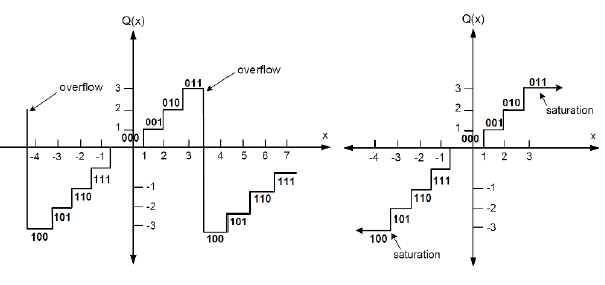
\includegraphics[width=\columnwidth]{Images/saturation}
\end{center}

\textbf{Beispiel} Multiplikation
\begin{lstlisting}
-- fixed_pkg
signal sMultiplicand : sfixed(1 downto -2) := to_sfixed(S_MULTIPLICAND, 1, -2); -- sQ2.2
signal sMultiplier : sfixed(1 downto -2) := to_sfixed (S_MULTIPLIER, 1, -2); -- sQ2.2
signal sProduct : sfixed(3 downto -4); -- Q4.4 -> Q(n1+n2).(m1+m2)

-- sProduct has two sign bits
sProduct <= sMultiplicand * sMultiplier;
-- If second sign bit shall be removed: Q3.4 -> Q(n1+n2-1).(m1+m2)
signal sProductShort : sfixed(2 downto -4);
-- sProductShort has only one sign bit
sProductShort <= resize(sProduct,2,-4);
\end{lstlisting}

\subsubsection{Limits}
\begin{center}
	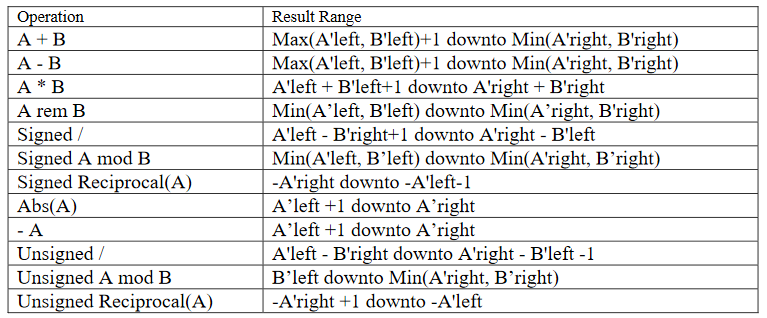
\includegraphics[width=\columnwidth]{Images/limits}
\end{center}

Addition:
\[
Q(n1,m1) + Q(n2,m2) = Q(\max(n1, n2) + 1, \max(m1, m2))
\]
Multiplikation
\[
Q(n1,m1) \cdot Q(n2,m2) = Q(n1 + n2, m1 + m2)
\]
Für signed * signed: MSB ist redundant
\[
Q(n1,m1) \cdot Q(n2,m2) = Q(n1 + n2 -1, m1 + m2+1)
\]